\section{Hybrid Dynamical Systems\label{sec:HD_systems}}
%
The basic notions of hybrid dynamical system and their hybrid inclusions formulation will be now defined. Part of the content of this Section is inspired by \cite{goebel2009hybrid,Goebel2012}.

Hybrid dynamical systems represent a wide class of systems in which continuous time and discrete time dynamics interacts. In recent years, there has been a growing interest in this field. One of the main reason is that these kind of systems provide a new and promising modeling perspective for systems presenting discontinuous behaviors as well as multimodality. The presence of both discrete and continuous dynamics makes this formalism appealing also for modeling physical phenomena in many different areas, from biology and medical applications to robotics, manufacturing, traffic management and bio-molecular networks~\citep{Aihara4893, Bortolussi2018}. 
Overviews of this framework are given in ~\citep{van2000introduction, haddad2006impulsive,goebel2009hybrid,Goebel2012}.
%
\subsection{Hybrid Inclusions}
%
Hybrid Inclusions are the most general formulation in the hybrid systems framework. They are made up with a constrained differential inclusion and a constrained difference inclusion in the form:
\begin{equation}\label{eq:hs}
%
\left\{ 
\begin{matrix*}[l]\vspace{1pt}
%
\dot{\xb} \in \F(\xb,\ub_c) &&(\xb,\ub_c)\in\C\times\U_c\\
\xb^+ \in \G(\xb,\ub_d)&&(\xb,\ub_d)\in\D\times\U_d
%
\end{matrix*}
\right.
%
\end{equation}
%
with state $\xb\subseteq\R^n$, inputs $\ub_c\in\U_c\subseteq\R^{m_c}$, $\ub_d\in\U_d\subseteq\R^{m_d}$ acting during \textit{flows} and \textit{jumps} respectively. ${\F}:\R^n\times\R^{m_c}\rightrightarrows\R^n$, $\G:\R^n\times\R^{m_d}\rightrightarrows\R^n$ are set--valued mappings and $\C$, $\D$ are subsets of $\R^n$ with. Let us call $\C$ the \textit{flow set}, $\F$ the \textit{flow map}, $\D$ the \textit{jump set} and $\G $ the \textit{jump map}.
%
\newline

%
The trajectories resulting from this kind of systems are defined on a \textit{hybrid time domain}. In fact, given the dual nature of hybrid systems (continuous and discrete), to parametrize its solutions both a continuous time $t$ and an discrete time $k$ are needed.
%
\begin{defn}[Hybrid time domain]
    Let $\E$ be a subset of $\R^+\times\mathbb{N}$, i.e. $\E\subset\R^+\times\mathbb{N}$. $\E$ is a compact hybrid time domain if 
    %
    \begin{equation}
        \E\triangleq\bigcup_{k = 0}^{j-1}\left[t_k,t_{k+1}\right]\times {k} 
    \end{equation}
    %
    such that
    %
    \begin{equation}
        t_0 = 0~~\land~~\forall k\leq j~t_k\leq t_{k+1}~
    \end{equation}
    %
    and one of the following hold:
    \begin{itemize}
        \item [i)] there are infinite intervals, i.e. $j = \infty$;
        \item [ii)] $j<\infty$ and the last interval is of the form
        \begin{equation}
            \left[t_{j-1},t_f\right)\times \{j\}~~\text{with}~~t_f<\infty~\lor~t_f = \infty
        \end{equation}
    \end{itemize}
    %
\end{defn}
%
The solutions of (\ref{eq:hs}) are definite on \textit{hybrid arcs} and parametrized by an hybrid time domain $\E$. The technical details of this formulation are discussed in \citep{Goebel2012}. 
%
\begin{exmp}[ball bouncing on actuated surface]
    %
    Consider a ball bouncing on an mechanically actuated surface which controls the speed of the ball after impacts. This example is inspired by \citep{naldi2013passivity}. A graphical representation of the system is show in Fig. \ref{fig:bb}.
    %
    \begin{figure}[h]
        \centering
        \definecolor{ocean}{rgb}{0.00000,0.44700,0.74100}
\begin{tikzpicture}
	% platform
	\fill[ocean!50, draw = black,thick] (-.75,0) rectangle (.75,0.2);
	% ball
	\fill[gray!25, draw=black,thick] (0,1.5) circle (0.5);
	% ground
	\draw[pattern=north east lines] (-2,0) rectangle (2,-.3);
	% labels	
	\draw[thick,->] (0,1) -- (1,1) -- (1,1.5) node[anchor=west] {$q$};
	\node at (-1,0.15) {$u$};
	\node at (0,1.5) {$m$};
	%
\end{tikzpicture}
        \caption[Ball bouncing on an actuated surface]{Ball bouncing on an actuated surface.}
        \label{fig:bb}
    \end{figure}
    %
    Let $q$ be the height of the ball from the ground, $v\triangleq\dot{q}$ be its velocity and let $\xb\triangleq(q,v)$. While the ball is ``flying'', the dynamic of the systems are just the one of a falling rigid body in a fluid of viscosity $\beta>0$ due to gravity ($\gamma=9.81$):
    %
    \begin{equation}
        \left\{
            %
            \begin{matrix*}[l]
                %
                \dot{q} = v\\
                %
                \dot{v} = -\gamma-\frac{\beta}{m}v
                %
            \end{matrix*}
            %
        \right.
    \end{equation}
    %
    and, thus
    %
    \begin{equation}
        \dot{\xb} = \F(\xb)\triangleq
        %
        \begin{bmatrix}
            0&1\\
            0&-\beta/m
        \end{bmatrix}\xb + 
        %
        \begin{bmatrix}
            0\\
            -\gamma
        \end{bmatrix}
        %
        \quad \text{if}\quad \xb\in\C\triangleq\left\{\xb:q\geq 0\right\}\setminus\left\{\xb:q=0\land v\leq 0\right\}.
        %
    \end{equation}
    %
    When the ball hits the actuated surface, the impact is modeled as
    %
    %
    \begin{equation}
        \left\{
            %
            \begin{matrix*}[l]
                %
                q^+ = q\\
                %
                v^+ = (u-c)v
                %
            \end{matrix*}
            %
        \right.
        %
        \quad c\in(0,1)
    \end{equation}
    %
    and, thus
    %
    \begin{equation}
        \xb^+ = \G(\xb,u)\triangleq
        %
        \begin{bmatrix}
            1&0\\
            0&u-c
        \end{bmatrix}\xb
        %
        \quad \text{if}\quad (\xb,u)\in\D\times\U_d\triangleq\left\{\xb:q=0\land v\leq 0\right\}\times\R.
        %
    \end{equation}
    %
    The final hybrid system is 
    %
    \begin{equation}
            \left\{
            %
            \begin{matrix*}[l]
                %
                \dot{\xb} = \F(\xb) &\xb\in\C\\
                %
                \xb^+ = \G(\xb,u) &\xb\in\C\times\U_d
                %
            \end{matrix*}
            %
        \right.
    \end{equation}
    %
    Note that the energy of the system is $\Ha(\xb) = \frac{m}{2}v^2 + m\gamma q$.
    %
    A numerical simulation of the autonomous system $u=0$ is given with $m=1$, $\beta = 0.1$, $c=0.9$ and $\xb=(1,0)$. The resulting trajectory is shown in Fig. \ref{fig:bb1}
    %
    \begin{figure}
        \centering
        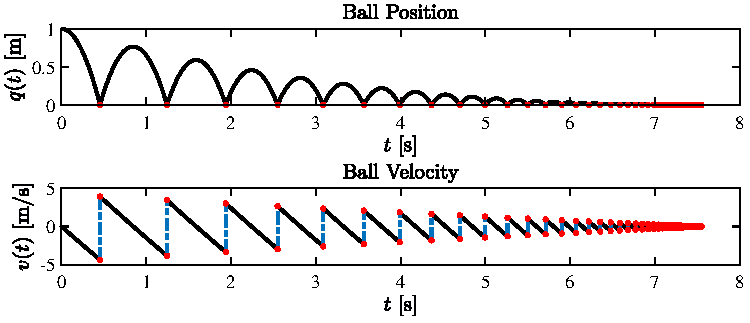
\includegraphics[width=\linewidth]{Figures/bb1.pdf}
        \caption[Time evolution of the ball bouncing on the actuated platform (autonomous case)]{Time evolution of the ball bouncing on the actuated platform (autonomous case).}
        \label{fig:bb1}
    \end{figure}
    %
\end{exmp}
%
%\begin{exmp}[Sliding mode controller]
%\textcolor{red}{to be completed...}
%\end{exmp}
%
\subsection{Stability}
%
Lyapunov stability theorems has been indeed extended to the hybrid case. In the case of continuous--time dynamical systems, the stability of equilibrium points is usually discussed. However, in case of hybrid systems, it is rather convenient to analyze the stability of a set. Hereafter the very basic results on Lyapunov stability of hybrid systems will be introduced.
%
\begin{thm}[Lyapunov Stability for Hybrid Systems \citep{goebel2009hybrid}]\label{thm:hybrid_Lyap}
	%
	Let us consider an autonomous hybrid system $\left(\C,\F,\D,\G\right)$ and a compact set $\A\subset\R^n$ satisfying $\G\left(\D\cap\A\right)\subset\A$. If there exists a Lyapunov function candidate $V:\C\cup\D\rightarrow\R$ such that:
	\begin{subequations}
		\begin{align}
		&V(\xb)>0&&\forall \xb\in \left(\C\cup\D\right)\setminus\A\label{eq:stabh_1}\\
		&\langle\frac{\partial V}{\partial \xb},\mathbf{f}(\xb)\rangle\leq 0&&\forall \xb\in\C\setminus\A,\mathbf{f}\in\F\label{eq:stabh_2}\\
		&V(\mathbf{g}(\xb)) - V(\xb)\leq 0 &&\forall \xb\in\D\setminus\A,\mathbf{g}\in\G\label{eq:stabh_3}
		\end{align}
	\end{subequations}
	%
	then the set $\A$ is stable.
\end{thm}
%
\begin{cor}[\cite{goebel2009hybrid}]$\newline$
	Let $\Gamma_\mu := \left\{x\in\C\cup\D:V(x) = \mu\right\}$. If there exists a compact neighborhood $\K$ of $\A$ such that, for all $\mu>0$, no solution of the system remains in $\Gamma_\mu\cap\K$, then the set $\A$ is pre-asymptotically stable. In this case the basin of pre-attraction contains every compact set contained in $\K$ that is forward invariant.
\end{cor}
%
\begin{exmp}[Ball bouncing on actuated platform]
Let consider the autonomous case (u=0) and let 
%
\begin{equation}
    \A\triangleq \left\{(q,v)~:~q\leq\delta q\in\R^+\land |v|\leq\delta v\in\R^+\right\}.
\end{equation}
%
Indeed it holds 
%
\begin{equation}
    \A\cap\D = \left\{(0,v)~:~v\leq 0\land |v|\leq\delta v\in\R^+\right\}
\end{equation}
%
and
%
\begin{equation}
    \G\left(\A\cap\D\right) = \left\{(0,-cv)~:~v\leq 0\land |v|\leq\delta v\in\R^+\right\}\subset \A.
\end{equation}
%
Let's examine the stability of $A$. By choosing as Lyapunov function the energy of the system: $V(\xb) = \Ha(\xb)$. It holds, $\Ha(\xb)>0~~\forall \xb\in\left(\C\cup\D\right)\setminus\A$ and
%
\begin{align}
    \langle\frac{\partial\Ha}{\partial \xb},\F(\x)\rangle &= [m\gamma,mv]\begin{bmatrix}0&1\\0&-\beta/m\end{bmatrix}\begin{bmatrix}q\\v\end{bmatrix} + [m\gamma,mv] \begin{bmatrix}0\\-\gamma\end{bmatrix} \\
    & = -\beta v^2 \leq 0\quad\forall v\in\R
\end{align}
%
which indeed holds for all $\xb\in\C\setminus\A$.
%
Finally, stability of $\A$ is proving noticing that
%
\begin{align}
    \Ha(\x^+) -\Ha(\xb) &= \frac{m}{2}(v^+)^2 + m\gamma q^+ - \frac{m}{2}v^2 + m\gamma q\\
    &= \frac{m}{2}(c-1)v^2\leq 0 \quad\forall v\in\R,~\forall c\in(0,1)
\end{align}
%
which holds also for any $\xb\in\D\setminus\A$. Note that in the case of the controlled system, $\A$ remains Lyapunov stable if and only if for all $t\geq 0$, $u(t)\leq c$. The descent of the energy during a trajectory of the system is represented in Fig. \ref{fig:bb2}
%
\begin{figure}[!h]
    \centering
    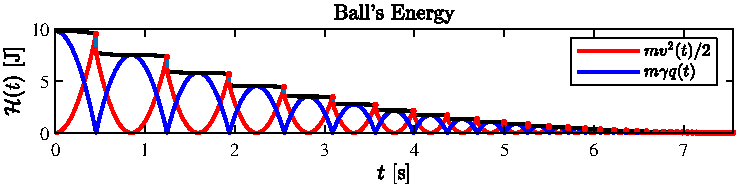
\includegraphics{Figures/bb2.pdf}
    \caption{Energy Descent during trajectory a trajectory of the autonomos system.}
    \label{fig:bb2}
\end{figure}
%
\end{exmp}
%
% \begin{exmp}[Sliding mode controller]
% \textcolor{red}{to be completed...}
% \end{exmp}
%
\clearpage